\ifspanish

\question Las siguientes verosimilitudes caracterizan un problema de decisión binario bidimensional con  $P_H(0)=3/5$:
\begin{align*}
p_{X_1,X_2|H}(x_1,x_2|0) &= 2,                      & 0<x_1<1, \quad 0<x_2<1-x_1  \\
p_{X_1,X_2|H}(x_1,x_2|1) &= 3\left( x_1+x_2\right), & 0<x_1<1, \quad 0<x_2<1-x_1 
\end{align*}

  
\begin{figure}[h]
\begin{center}
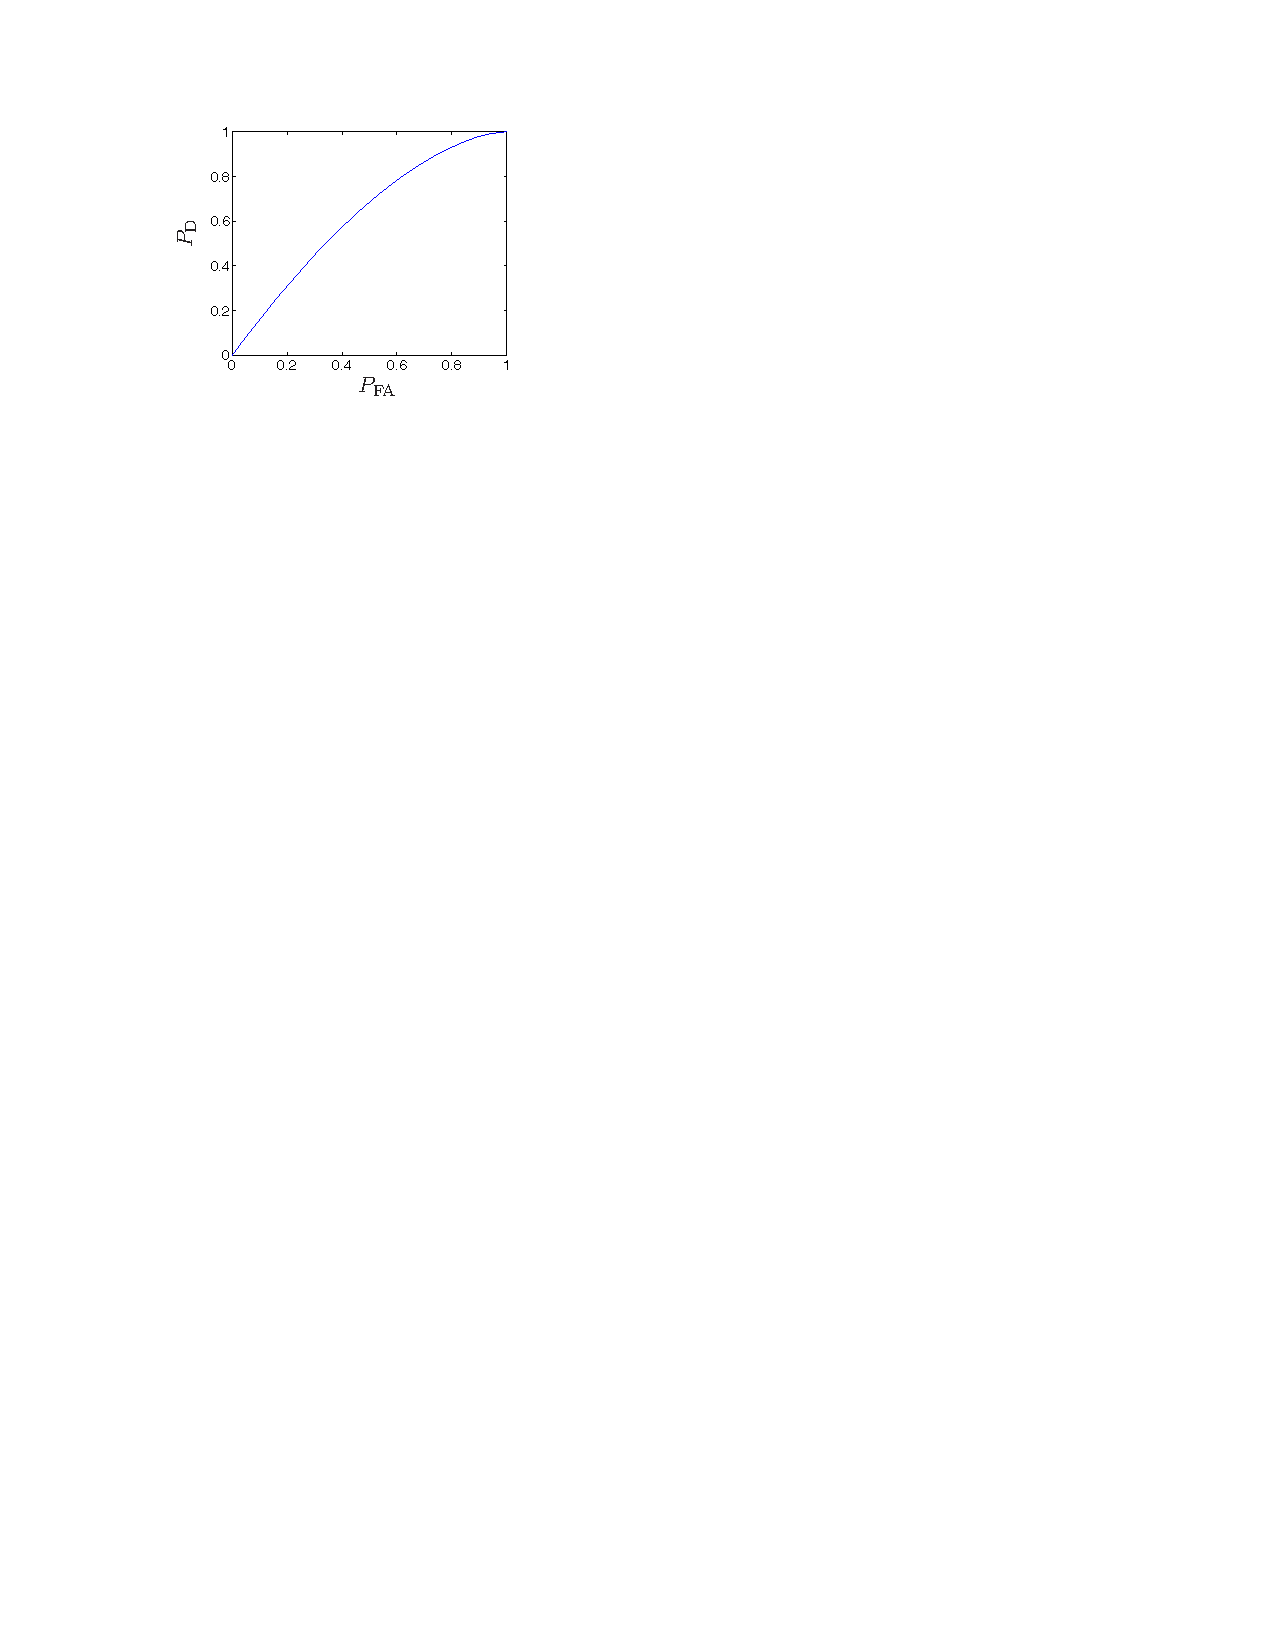
\includegraphics[width=14cm, trim=0cm 22cm 7cm 2cm]{Figuras/ROC}
\end{center}
\end{figure}

Considérese un decisor LRT genérico con umbral $\eta$,
\begin{parts}
\part Calcúlese la $P_{\rm FA}$ en función de $\eta$.
\part La siguiente figura representa la ROC {del LRT}.  Justificando su respuesta:
\begin{itemize}
\item {Indique} sobre la {ROC} cómo varía el punto de trabajo del decisor al aumentar o disminuir el umbral del test.
\item {Situe} sobre la {ROC} los puntos de trabajo correspondientes al decisor ML, al decisor de mínima probabilidad de error y al decisor de Neyman-Pearson con $P_{\rm FA} = 0.3$.
\end{itemize}

\end{parts}

\begin{solution}
\begin{parts}
\part $x_1+x_2 \dunodcero \dfrac{2}{3}\eta =\eta'  \quad \quad P_{\rm FA}=1-\eta'^2$
\part \begin{itemize}
\item $P_{\rm FA}$ y $P_{\rm D}$  decrecen al aumentar el umbral
\item
 	Decisor ML: $\eta=1$, $\eta'=\dfrac{2}{3}$, $P_{\rm FA}=\dfrac{5}{9}$.\\
	Decisor MAP: $\eta=\dfrac{3}{2}$,	$\eta'=1$,	$P_{\rm FA}=0$.\\
	Decisor N-P:	$P_{\rm FA}=0.3$.
	\end{itemize}
\end{parts}
\end{solution}

\else

\question The following likelihoods characterize a bidimensional binary decision problem with $P_H(0)=3/5$:
\begin{align*}
p_{X_1,X_2|H}(x_1,x_2|0) &= 2,                      & 0<x_1<1, \quad 0<x_2<1-x_1  \\
p_{X_1,X_2|H}(x_1,x_2|1) &= 3\left( x_1+x_2\right), & 0<x_1<1, \quad 0<x_2<1-x_1 
\end{align*}
 
\begin{figure}[h]
\begin{center}
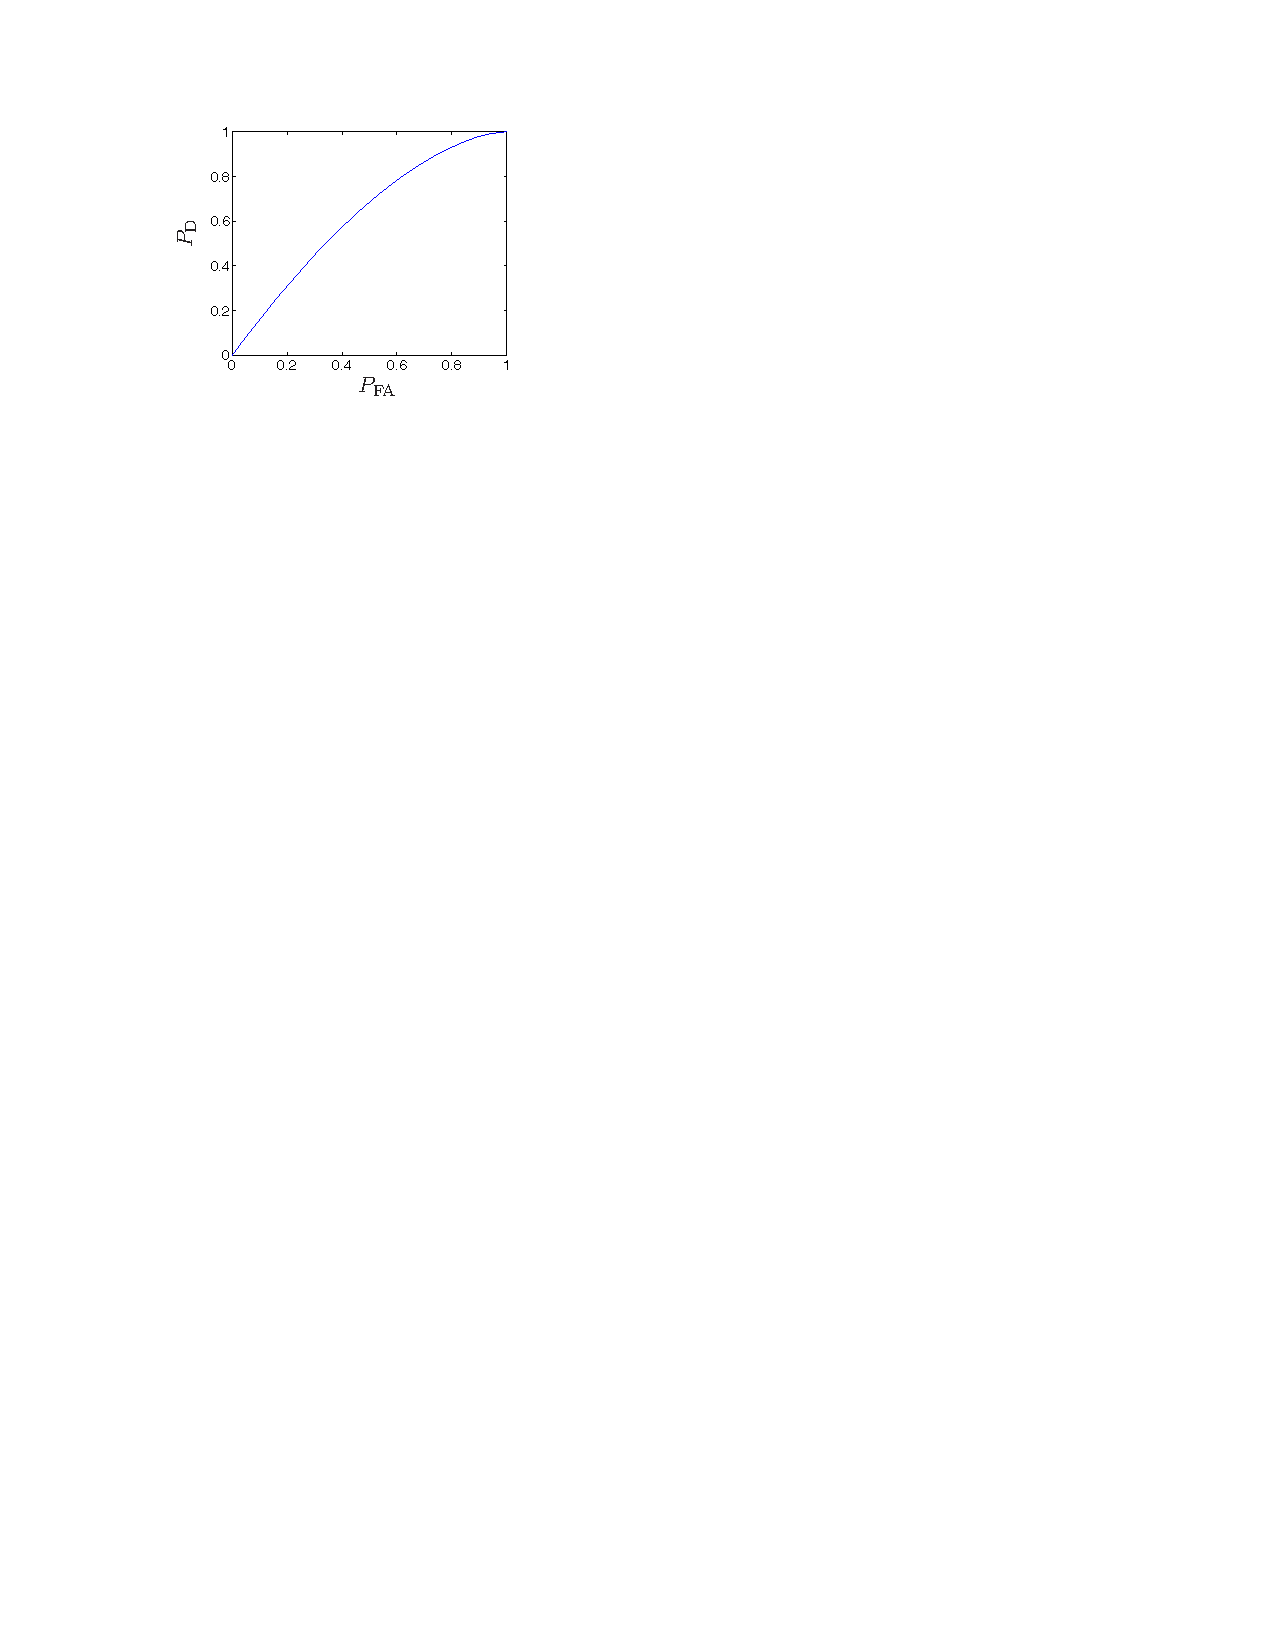
\includegraphics[width=14.5cm, trim=0cm 21.5cm 7cm 2cm]{Figuras/ROC}
\end{center}
\end{figure}

Consider a generic LRT decision maker with threshold $\eta$,
\begin{parts}
\part Calculate $P_{\rm FA}$ as a function of $\eta$.
\part The figure represents the ROC curve of the LRT. Justifying your answer:
\begin{itemize}
\item Indicate on the ROC how the operation point moves on the curve when increasing or decreasing the threshold of the test.
\item Place on the ROC the operation points corresponding to the ML classifier, to the decision maker with minimum probability of error, and to the Neyman-Pearson detector with $P_{\rm FA} = 0.3$.
\end{itemize}
\end{parts}

\begin{solution}
\begin{parts}
\part $x_1+x_2 \dunodcero \dfrac{2}{3}\eta =\eta'  \quad \quad P_{\rm FA}=1-\eta'^2$
\part \begin{itemize}
\item $P_{\rm FA}$ and $P_{\rm D}$ decrease as the threshold is increased.
\item
ML classifier: $\eta=1$, $\eta'=\dfrac{2}{3}$, $P_{\rm FA}=\dfrac{5}{9}$.\\
MAP classifier: $\eta=\dfrac{3}{2}$,	$\eta'=1$,	$P_{\rm FA}=0$.\\
N-P decision maker:	$P_{\rm FA}=0.3$.
	\end{itemize}
\end{parts}

\end{solution}

\fi